\expandafter\ifx\csname ifdraft\endcsname\relax
 \begin{document}
\fi

\section{検証}

計算の章(\ref{sec:calculation})で述べたように,多くの各種計算値は酸素摂取量VO_2を元に算出される.そこで,今回は実験により酸素摂取量を測定することで装置の検証を行う.

なお,今回の検証は新型コロナウィルス感染症緊急事態宣言中に行った.呼吸代謝測定装置はマスク部などに唾液が多く付着するため,感染防止の観点から複数人の被験者を対象にした実験を行うことが難しい.よって,実験は筆者が自宅にて自身一人を被験者として行っている.ご了承いただきたい.

酸素摂取量の測定には,トレッドミルや自転車エルゴメーター,踏み台などが用いられる.今回は自宅で実験を行うため,パワーメーター(出力計)を装着したロードバイクを自動負荷調整機能付きのローラー台に取り付けて検証を行った.
検証はパワーを指定したワークアウトを作成し,ワークアウト中の酸素摂取量に加えて,ロードバイクや身体に取り付けたセンサーによって実際のパワー,心拍数,ケイデンス(ペダル)回転数を測定する.

様々な点で装置の検証を行うため,以下の3つの実験を行った.

\begin{enumerate}
  \item ランプアップ・ダウン
  \item 最大酸素摂取量測定
  \item 負荷変動を伴うワークアウト
\end{enumerate}

以上の実験を行った上で,装置が出力するログデータとその他のセンサーで測定したデータをタイムスタンプを用いて統合して検証を行う.

\subsection{実験方法}

今回,酸素摂取量は一般的な指標となっていることから1分あたりの体重あたり酸素摂取量(mL/kg/min)を使用する.体重は実験直前に測定し装置のプログラムに書き込む.
諸条件の変化を最小限にするため実験は室内で行った.実験中に空気の組成の変化を最小限にするため,実験開始の1時間以上前から部屋の窓を解放した.また,ロードバイクのパワーメーターは温度変化の影響を抑えるため,窓を解放した部屋にあらかじめ置いておき,実験の直前に校正を行った.
また,ミキシングチャンバー内が確実に換気されるようにミキシングチャンバーから
その上で,ロードバイクのパワーメーターの校正と装置の酸素センサーA-5Sの校正を行い,

実験手順をまとめると以下の通りである.

\begin{enumerate}
  \item 実験開始1時間以上前に部屋の窓を開ける
  \item ロードバイクのパワーメーターを校正する
  \item 装置の酸素センサーA5-Sを大気中の酸素濃度の値に校正する
  \item 装置の電源を入れてデータの記録が開始する
  \item マスクを装着する
  \item ワークアウトを開始する
  \item ワークアウトを終了する
  \item 装置の電源を切ってデータの記録が終了する
  \item Micro SDカードからデータを取り出す
\end{enumerate}

本研究で製作した装置は各値の算出に1分平均値を使用しているため,マスクを装着後1分間のデータは除外する必要がある.そのためウォーミングアップを兼ねて5分間,最初の設定パワーでペダリングを続けるようにしている.

\end{enumerate}

\subsection{実験機材}

今回使用したパワーメーターは,4iiii InnovationsのPrecision 2.0 3Dである.自転車運動のパワーを測定する方法は複数あるが,このパワーメーターは左側のクランクアームの裏側に貼り付けた歪みゲージによって計測されたトルクと,加速度センサーによって計測されたケイデンス(ペダル回転数)からパワーを算出する一般的なタイプである.算出されたパワー値はANT+またはBluetoothによってサイクルコンピューターやパソコンなどに無線で送信される.

自動負荷調整機能付きローラー台とは,自転車を取り付けて漕いだ時に実走のような負荷を作り出すローラー台の中でも,サイクルコンピューターやパソコンなどから送信される信号に応じて負荷の強さを調整する機能を備えたもののことである.今回はGROWTACのハイブリッド式(前輪固定式)ローラー台のGT-ROLLER Flex3に同社の自動負荷調整装置であるGT-ePower-FとGT-eBoxを取り付けて自動負荷調整機能付きローラー台として使用した.

今回の実験は,これらの機材を用いてあらかじめ設定したパワーで自転車運動を行った際の酸素摂取量を測定することで行った.その際にパワーやケイデンス,継続時間を設定したワークアウトを作成し運動を行うためにZwiftを用いた.Zwiftはバーチャルワールド内を自転車に乗ったアバターを操作して走ることができるバーチャルサイクリングプラットフォームである.地形に応じて負荷が変動する機能が特徴だが,ワークアウト中には一定負荷,またはERGモードと呼ばれ右自動負荷モードになる.ERGモードは設定パワーに合わせて負荷を調整することで,いかなるケイデンスでペダリングしてもパワーが設定パワーに一定に保たれるというモードである.今回の実験では,設定パワーに応じた負荷量がローラー台の最低負荷量を下回ることでERGモードが停止する実験1を除いて,ERGモードを使用して行っている.

心拍数を測定するためにScoscheの光学式心拍計のRHYTHM+を使用した.光学式心拍計は皮膚に光を照射し,血管内の反射を読み取ることで脈拍を計測する.この心拍計は光源に3つのLED(緑色2個,黄色1個)を使用している.本来は前腕内側に巻きつけることが推奨されているが,普段の使用で皮下脂肪量が多い上腕外側に巻きつけて使用した方が異常値の出力の頻度が低くなることが確認できているため上腕外側に巻きつけて心拍数を計測した.

\begin{figure}[h]
  \begin{center}
    \label{fig:gt-roller_flex3}
    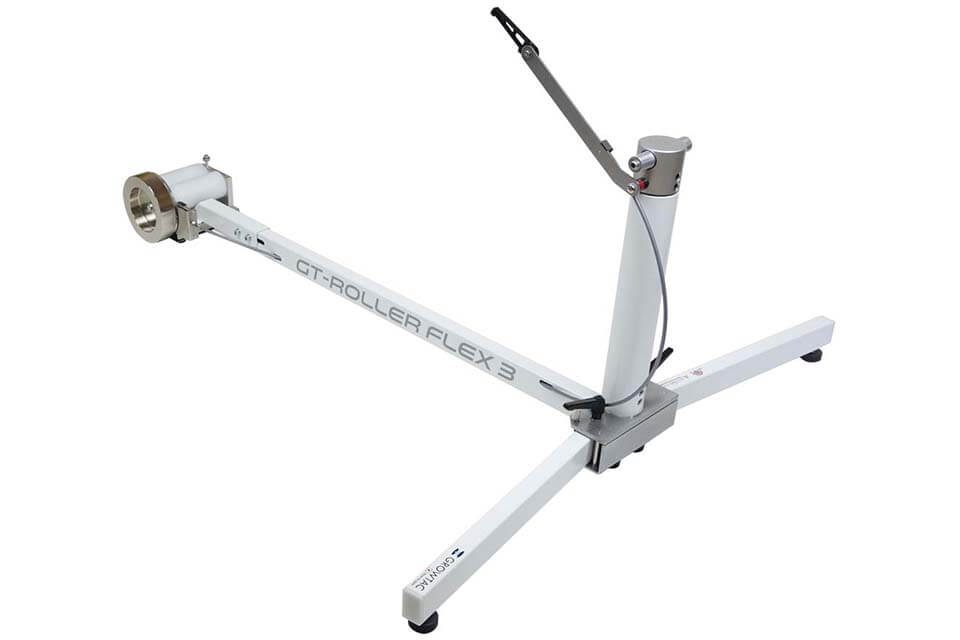
\includegraphics[width=8cm]{fig/gt-roller_flex3.jpg}
    \caption{GT-Roller Flex3(写真は手動負荷調整装置付き)}
  \end{center}
\end{figure}

\subsubsection{データの取得}

製作した装置が記録したデータはMicro SDカード上のcsvファイルに書き込まれる.データは取得間隔1秒でタイムスタンプが付与されている.一方,ロードバイクに取り付けたパワーメーターや

\subsection{ランプアップ・ダウン}

\subsubsection{実験方法}

最大酸素摂取量(VO_2Max)以下の低強度で自転車を漕ぐ時,パワーが高いほど酸素摂取量が多くなるはずである.酸素摂取量とパワー,心拍数を比較することで酸素摂取量の変化を調べる.

ケイデンスを一定に保ち(今回は慣例に従い60rpmとした)ペダリングをし,設定パワーを一定段階で引き上げたあと,一定段階で引き上げるという実験を行い,設定パワーと酸素摂取量パワーを上げた時と

製作した装置は1分平均値を用いて計算を行うため,運動開始1分間のデータは除外する必要がある.このため設定パワーでの運動に入る前に,ウォーミングアップを兼ねて40Wで5分間ペダリングをした後に,3分ごとに設定パワーを40Wずつ3段階引き上げる.その後に3分ごとに

また,それぞれの実験は別の日に行った.

低強度,高強度のそれぞれの設定パワーは以下の図の通りである.

\begin{enumerate}
  \item 5分間ウォーミングアップを兼ねて40W
  \item 3分ごとに40Wずつ3段階設定パワーを上げる
  \item 3分ごとに40Wずつ3段階設定パワーを下げる
  \item 5分間40W
\end{enumerate}

\begin{figure}[h]
  \begin{center}
    \label{fig:protocol_rampup_light}
    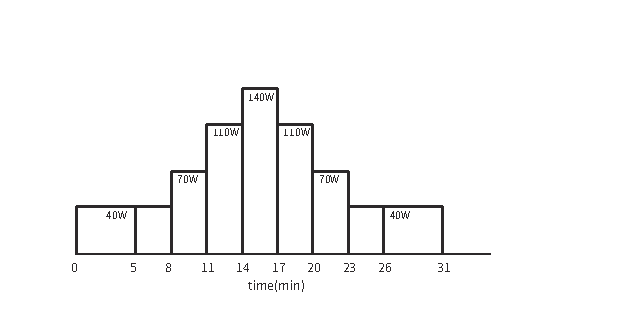
\includegraphics[width=10cm]{fig/protocol_rampup_light.pdf}
    \caption{ランプアップ・ダウン(低強度)}
  \end{center}
\end{figure}

\begin{figure}[h]
  \begin{center}
    \label{fig:protocol_rampup_hard}
    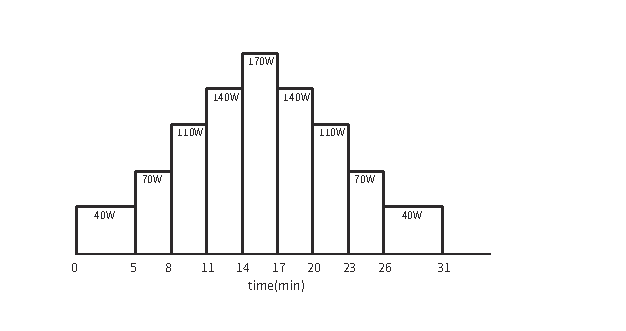
\includegraphics[width=10cm]{fig/protocol_rampup_hard.pdf}
    \caption{ランプアップ・ダウン(高強度)}
  \end{center}
\end{figure}

\subsubsection{実験条件}

\begin{table}[h]
  \begin{center}
  \caption{ランプアップ・ダウン(低強度)}
  \label{tb:YFS201_specsheet}
    \begin{tabular}{ll}
      実験日 & 2021/01/24 \\
      開始時刻 & 10:30:46 \\
      体重 & 55.0kg \\
      気温(平均) & 12mm \\
      大気圧(平均) & 1-30L/min \\
      飽和水蒸気圧(平均) & 1L_{水} = 450pulse \\
      STPD係数(平均) & 1L_{水} = 450pulse
    \end{tabular}
  \end{center}
\end{table}

\begin{table}[h]
  \begin{center}
  \caption{ランプアップ・ダウン(高強度)}
  \label{tb:YFS201_specsheet}
    \begin{tabular}{ll}
      実験日 & 2021/01/25 \\
      開始時刻 & 9mm \\
      体重 & 55.0kg \\
      気温(平均) & 12mm \\
      大気圧(平均) & 1-30L/min \\
      飽和水蒸気圧(平均) & 1L_{水} = 450pulse \\
      STPD係数(平均) & 1L_{水} = 450pulse
    \end{tabular}
  \end{center}
\end{table}

\subsection{最大酸素摂取量測定}

\subsubsection{実験プロトコル}

\subsubsection{実験条件}

\subsection{負荷変動を伴うワークアウト}

\subsubsection{実験プロトコル}

\subsubsection{実験条件}

\subsection{使用中の様子と所感}

\subsection{既存の呼吸代謝測定装置との比較}

\subsubsection{実験方法}

\subsubsection{結果}

\subsubsection{考察}

\expandafter\ifx\csname ifdraft\endcsname\relax
  \end{document}
\fi
